% Options for packages loaded elsewhere
\PassOptionsToPackage{unicode}{hyperref}
\PassOptionsToPackage{hyphens}{url}
%
\documentclass[
  12pt,
]{article}
\usepackage{amsmath,amssymb}
\usepackage{lmodern}
\usepackage{iftex}
\ifPDFTeX
  \usepackage[T1]{fontenc}
  \usepackage[utf8]{inputenc}
  \usepackage{textcomp} % provide euro and other symbols
\else % if luatex or xetex
  \usepackage{unicode-math}
  \defaultfontfeatures{Scale=MatchLowercase}
  \defaultfontfeatures[\rmfamily]{Ligatures=TeX,Scale=1}
  \setmainfont[]{Times New Roman}
\fi
% Use upquote if available, for straight quotes in verbatim environments
\IfFileExists{upquote.sty}{\usepackage{upquote}}{}
\IfFileExists{microtype.sty}{% use microtype if available
  \usepackage[]{microtype}
  \UseMicrotypeSet[protrusion]{basicmath} % disable protrusion for tt fonts
}{}
\makeatletter
\@ifundefined{KOMAClassName}{% if non-KOMA class
  \IfFileExists{parskip.sty}{%
    \usepackage{parskip}
  }{% else
    \setlength{\parindent}{0pt}
    \setlength{\parskip}{6pt plus 2pt minus 1pt}}
}{% if KOMA class
  \KOMAoptions{parskip=half}}
\makeatother
\usepackage{xcolor}
\usepackage[margin=2.54cm]{geometry}
\usepackage{graphicx}
\makeatletter
\def\maxwidth{\ifdim\Gin@nat@width>\linewidth\linewidth\else\Gin@nat@width\fi}
\def\maxheight{\ifdim\Gin@nat@height>\textheight\textheight\else\Gin@nat@height\fi}
\makeatother
% Scale images if necessary, so that they will not overflow the page
% margins by default, and it is still possible to overwrite the defaults
% using explicit options in \includegraphics[width, height, ...]{}
\setkeys{Gin}{width=\maxwidth,height=\maxheight,keepaspectratio}
% Set default figure placement to htbp
\makeatletter
\def\fps@figure{htbp}
\makeatother
\setlength{\emergencystretch}{3em} % prevent overfull lines
\providecommand{\tightlist}{%
  \setlength{\itemsep}{0pt}\setlength{\parskip}{0pt}}
\setcounter{secnumdepth}{5}
\ifLuaTeX
  \usepackage{selnolig}  % disable illegal ligatures
\fi
\IfFileExists{bookmark.sty}{\usepackage{bookmark}}{\usepackage{hyperref}}
\IfFileExists{xurl.sty}{\usepackage{xurl}}{} % add URL line breaks if available
\urlstyle{same} % disable monospaced font for URLs
\hypersetup{
  pdftitle={Pika Distribution and Population Trends at Niwot Ridge},
  pdfauthor={Jacob Freedman and Logan Dye},
  hidelinks,
  pdfcreator={LaTeX via pandoc}}

\title{Pika Distribution and Population Trends at Niwot Ridge}
\usepackage{etoolbox}
\makeatletter
\providecommand{\subtitle}[1]{% add subtitle to \maketitle
  \apptocmd{\@title}{\par {\large #1 \par}}{}{}
}
\makeatother
\subtitle{\url{https://github.com/ldye16/DyeFreedman_ENV872_EDA_FinalProject}}
\author{Jacob Freedman and Logan Dye}
\date{}

\begin{document}
\maketitle

\newpage
\tableofcontents 
\newpage
\listoffigures 
\newpage

\hypertarget{rationale-and-research-questions}{%
\section{Rationale and Research
Questions}\label{rationale-and-research-questions}}

The American Pika is a threatened small mammal endemic to alpine tundra
habitat in the Rocky Mountains and Sierra Nevadas. Climate change is a
growing threat worldwide, and is expected to have a particular impact on
high elevation habitats. Pikas are sensitive to both temperature and
changes in the water balance (impacted by seasonality of snowmelt), so
climate change could undoubtedly threaten their long-term viability. In
addition, as Pikas occupy habitat at the tops of mountain ridges, their
possible migration either northward or to higher ridges would involve
them crossing over lower elevation valleys. Their ability to do so is
unknown, which makes their possibility of survival even murkier
(National Wildlife Federation).

Niwot Ridge is one of the most heavily studied alpine areas in the Rocky
Mountains. It is home to multiple research projects, as it is both a
NEON and LTER Site. LTER researchers have gathered data on Pika
demography and climate over the past 15-20 years. We used public
datasets to answer multiple questions regarding trends in climate and
Pika populations at Niwot Ridge.

\begin{enumerate}
\def\labelenumi{\arabic{enumi}.}
\tightlist
\item
  Is temperature changing over time at Niwot Ridge?
\item
  Are Pika populations changing over time and is there a correlation
  between population changes and temperature changes?
\item
  Are Pika populations changing spatially over time? Are they seeking
  higher elevation sites?
\item
  An increase in zoonotic diseases is a well documented effect of
  warming temperatures. Is mite and flea prevalence in Pikas changing
  over time and with temperature?
\end{enumerate}

\newpage

\hypertarget{dataset-information-and-wrangling}{%
\section{Dataset Information and
Wrangling}\label{dataset-information-and-wrangling}}

Both climate and pika data was sourced from the Niwot Ridge LTER
website. All datasets are for public use and are available here:
\url{https://nwt.lternet.edu/data-catalog} Significant wrangling was
required to answer the research questions. The general process is
explained below for each research question.

Temperature changes over time:

Climate data was available from 2000 to 2018, but 2008 to 2018 were
selected as this time frame overlapped with the available pika data. The
dataset contained the site and device names, daily min, max, and avg air
temperature, relative humidity, barometric pressure, wind
speed/direction, solar radiation and soil temperature. We then used the
package ``zoo'' to interpolate NA values in the temperature data.

Pika population changes over time and in relation to temperature:

Pika data was available from 2008 to 2020, but 2008 to 2018 were
selected as this time frame overlapped with the available climate data.
The dataset contained the site, data, slope aspect, location of capture,
identification information, demography data, biological samples
collected and parasite presence. In order to estimate population over
time, annual pika captures were identified at Niwot Ridge. This required
eliminating recaptures within the same year. Captures without a ``tag
type'', meaning that they were not tagged and there was insufficient
information to rule it out as a recapture, were eliminated. Second,
observations where the tag type was recorded, but none of the tag
information (ear tag color or number code) was recorded, were
eliminated. Finally, the dataset was split into separate datasets for
each year and the number of unique tag IDs (PikaID) was found to derive
annual counts.

To prepare for our temperature and pika abundance regressions, it was
necessary to calculate mean annual temperature values. The interpolated
temperature dataset was grouped by year and then summarized by average
daily temperature to calculate annual means. A column of ``year number''
(e.g.~1 = 2008) was also generated to run both regressions.

Pika spatial distribution changes:

To assess spatial changes, observations without spatial attributes
(easting, northing) were eliminated. Mean annual pika locations were
determined by summarizing the easting and northing columns. Both
individual and mean annual locations were converted to spatial
dataframes using the NAD83 Zone 13N projected coordinate system.

Parasite Data:

To determine if there was a change in parasite abundance over time and
with changing temperatures, flea and ear mite data was isolated from the
overall pika demography data. The parasite data included flea
observations, fleas sampled, ear mite observations, and ear mites
sampled. For both flea observations and fleas sampled, the recorded
value was the number of fleas either observed on or sampled on an
individual pika. For ear mites sampled, the recorded values were binary.
A ``0'' was recorded when a pika was not sampled for ear mites, and a
``1'' was recorded when a pika was sampled for ear mites. For ear mites
observed, the data was categorical. The categories were ``N'' for none,
``L'' for low density, ``M'' for medium density, ``H'' for high density,
``NA'' for individuals whose data was not recorded in the main trapping
notebook, and ``NS'' for Pikas who were not sampled for mites in this
way. There are also a few instances of either a ``0'' or a ``1'' being
recorded and a single recording of ``N?''.

Once we had isolated the flea and ear mite data from the demography
data, we split the dataframe into two, one with only flea data and one
with only ear mite data.

For the flea data, we grouped by PikaID to isolate individual pikas that
were recaptured in a given year. The data was split by year to find the
mean value of fleas sampled and fleas observed per pika for each year.
The single-year dataframes were then merged to create one dataframe with
the average number of fleas observed and sampled per pika per year.

The same methodology was used to wrangle the mite data. However, since
the data was binary, either ``0'' or ``1'', the resulting ear mite
sampled column represented a proportion of captured pikas sampled for
ear mites. Generally, if ear mites were observed on a pika, they were
sampled. Thus, the proportion of pikas sampled for ear mites represents
the proportion of total pikas captured in a given year with ear mites
present.

For ear mite observed data, a different wrangling technique was used to
account for the categorical data. The NA, NS, 0, 1, and N? observations
were eliminated and observations with ear mite data were retained: N, L,
M, and H. The ear mite densities were grouped by year and summarized to
obtain an annual account for each density category. To account for the
different number of pika captures each year, the data was converted to
an annual proportion of each mite density.

In the final step, the flea and mite dataframes were joined into one
final parasite dataframe. The final parasite dataframe was then joined
to the climate dataframe and a column of ``year number'' (e.g.~1 = 2008)
was generated to prepare for analysis.

\newpage

\hypertarget{exploratory-analysis}{%
\section{Exploratory Analysis}\label{exploratory-analysis}}

To initially explore the data, two simple plots were created with linear
trendlines. Mean average temperature from 2000-2018 (Figure 1) and pika
captures per year from 2008-2020 (Figure 2) demonstrate some promising
patterns. Temperature appears to be increasing over time while pika
population appears to be in decline.

\begin{figure}
\centering
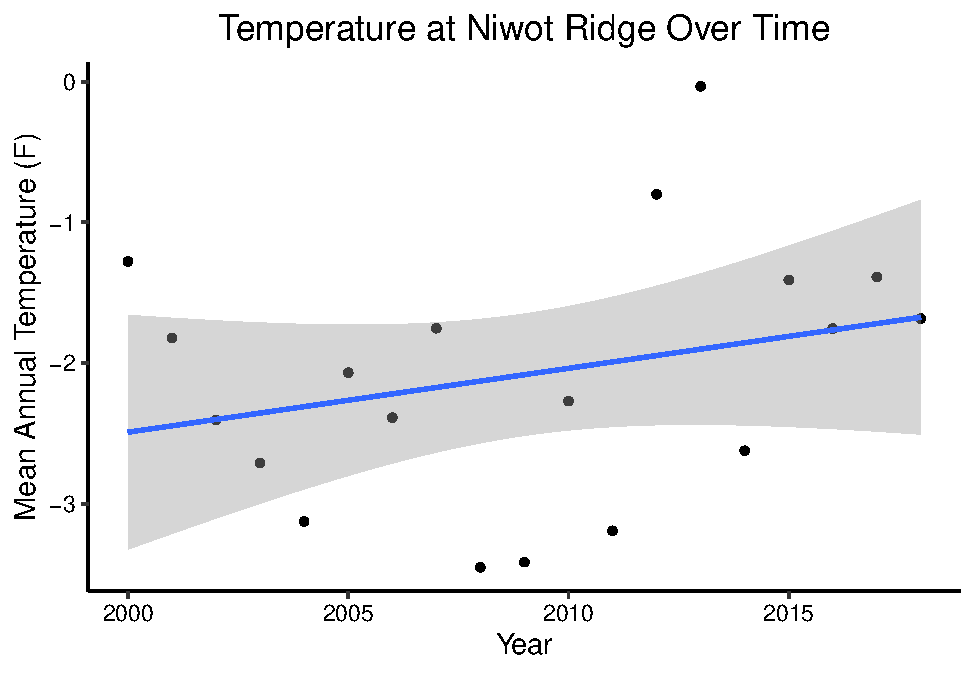
\includegraphics{FreedmanDye_ENV872_Project_files/figure-latex/unnamed-chunk-2-1.pdf}
\caption{Scatterplot of mean annual temperature at Niwot Ridge from 2000
to 2018.}
\end{figure}

\begin{figure}
\centering
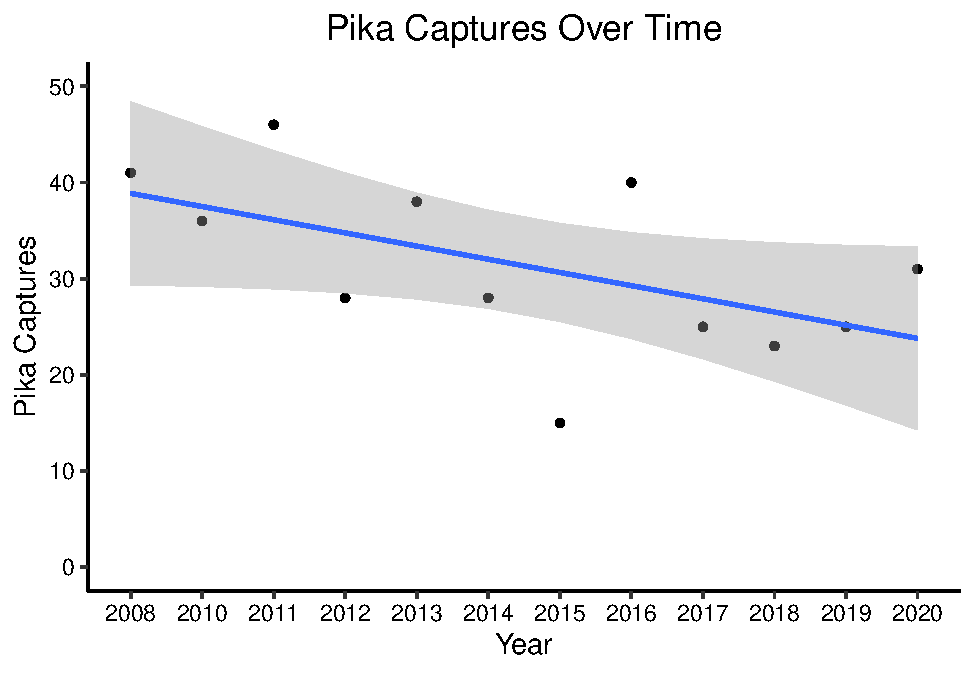
\includegraphics{FreedmanDye_ENV872_Project_files/figure-latex/unnamed-chunk-3-1.pdf}
\caption{Scatterplot of total annual pika captures at Niwot Ridge from
2008 to 2020.}
\end{figure}

\newpage

\hypertarget{analysis}{%
\section{Analysis}\label{analysis}}

\hypertarget{question-1-is-temperature-changing-over-time-at-niwot-ridge}{%
\subsection{Question 1: Is temperature changing over time at Niwot
Ridge?}\label{question-1-is-temperature-changing-over-time-at-niwot-ridge}}

A time series of daily average temperature was conducted from 2008 to
2018 to assess temperature changes over time. Temperature changed
significantly at Niwot Ridge (Seasonal Mann-Kendall, p-value =
6.133e-11). This is clear when examining the decomposed temperature data
(Figure 3), which despite the expected seasonality displays a trend of
increasing temperature. A plot of mean annual temperature also visually
reinforces these results (Figure 4).

\begin{figure}
\centering
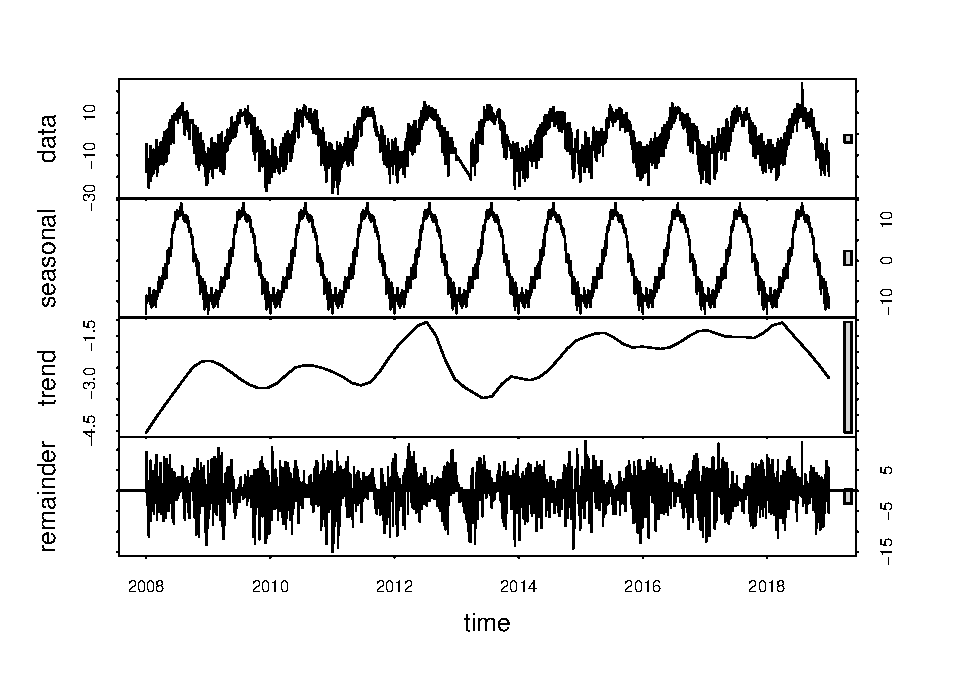
\includegraphics{FreedmanDye_ENV872_Project_files/figure-latex/unnamed-chunk-4-1.pdf}
\caption{Decomposed time series plot showing seasonal and overall
temperature trends at Niwot Ridge from 2008 to 2018.}
\end{figure}

\begin{figure}
\centering
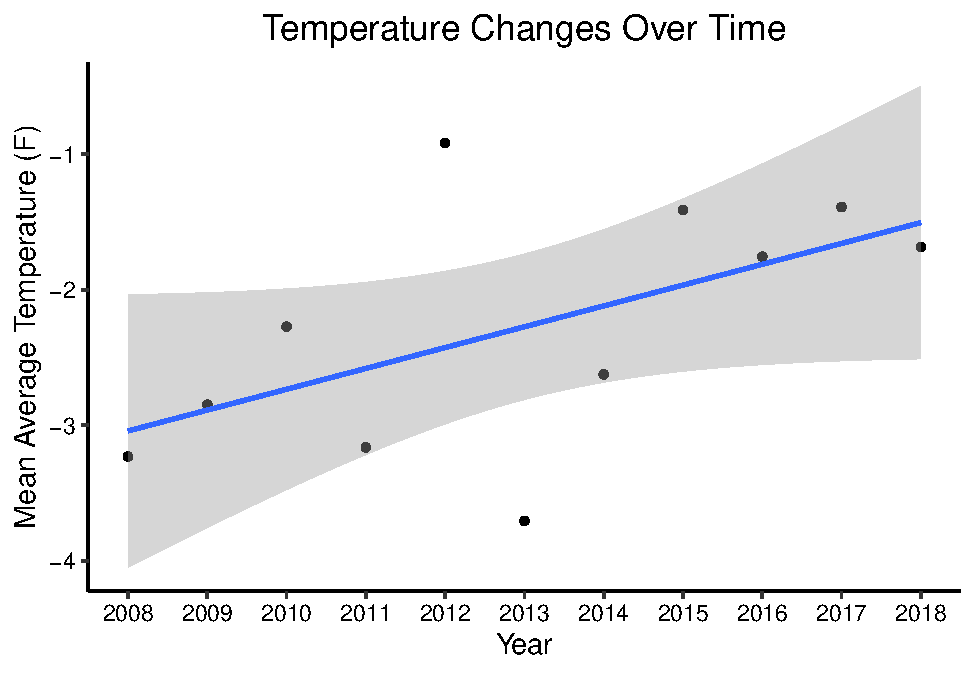
\includegraphics{FreedmanDye_ENV872_Project_files/figure-latex/unnamed-chunk-5-1.pdf}
\caption{Scatterplot of mean annual temperature at Niwot Ridge from 2008
to 2018.}
\end{figure}

\hypertarget{question-2-are-pika-populations-changing-over-time-and-is-there-a-correlation-between-population-changes-and-temperature-changes}{%
\subsection{Question 2: Are Pika populations changing over time and is
there a correlation between population changes and temperature
changes?}\label{question-2-are-pika-populations-changing-over-time-and-is-there-a-correlation-between-population-changes-and-temperature-changes}}

Linear regressions were conducted to analyze pika populations over time
and in relation to changing temperature. Annual pika populations did not
change significantly from 2008 to 2020 (Linear Model, F = 2.98, df = 10,
Adjusted R-squared = 0.1525, p-value = 0.115). However, the general
population trend appears to be decreasing (Figure 5) and it was found
that populations did decrease significantly in response to higher
temperatures (Linear Model, F = 6.396, df = 8, Adjusted R-squared =
0.3748, p-value = 0.0353, Figure 6).

\begin{figure}
\centering
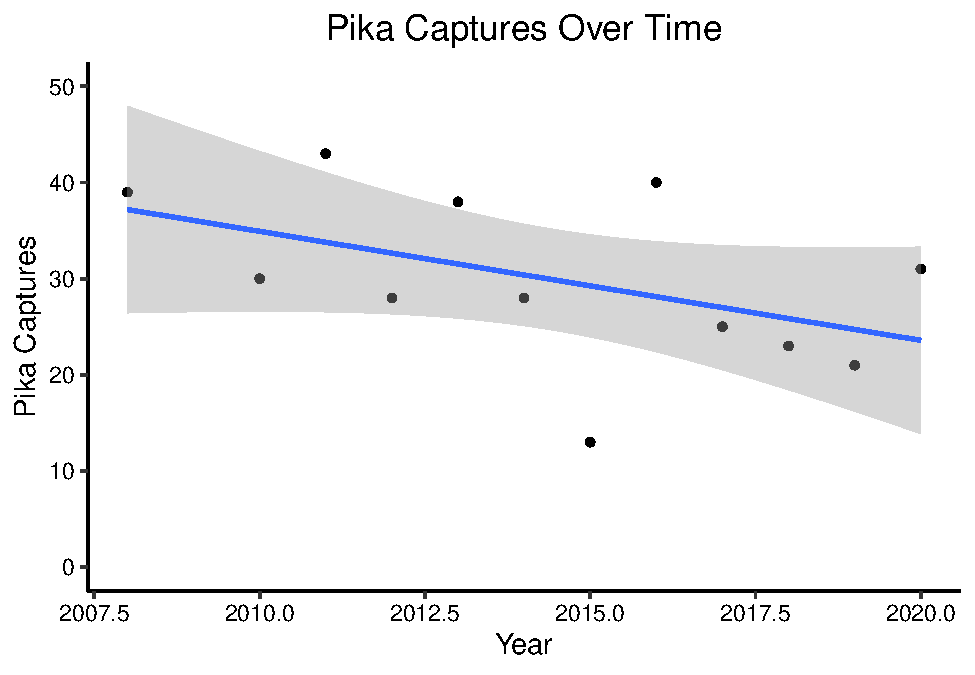
\includegraphics{FreedmanDye_ENV872_Project_files/figure-latex/unnamed-chunk-6-1.pdf}
\caption{Scatterplot of total annual pika captures at Niwot Ridge from
2008 to 2020.}
\end{figure}

\begin{figure}
\centering
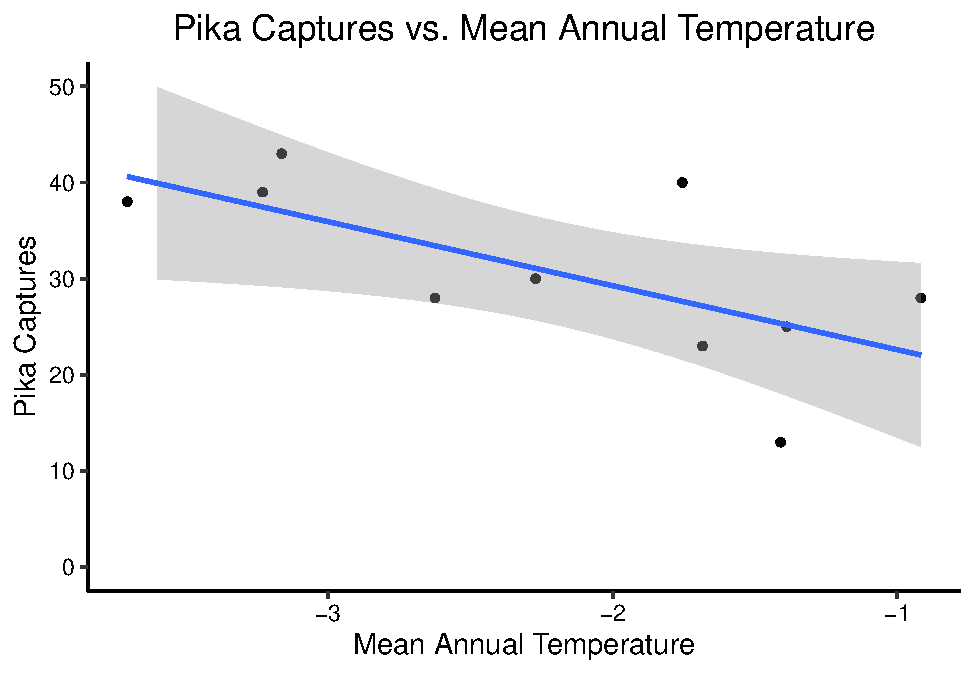
\includegraphics{FreedmanDye_ENV872_Project_files/figure-latex/unnamed-chunk-7-1.pdf}
\caption{Scatterplot of annual pika captures and mean temperature at
Niwot Ridge from 2008 to 2018.}
\end{figure}

\hypertarget{question-3-are-pika-populations-changing-spatially-over-time-are-they-seeking-higher-elevation-sites}{%
\subsection{Question 3: Are Pika populations changing spatially over
time? Are they seeking higher elevation
sites?}\label{question-3-are-pika-populations-changing-spatially-over-time-are-they-seeking-higher-elevation-sites}}

Spatial changes in pika population were estimated by calculating and
plotting the mean annual capture location. Figure 7 shows the mean
capture locations from 2008 to 2020, and Figure 8 shows all captures to
help better visualize the study area. There are three sampling sites
(Mitchell Lake to the North - 11,044 feet, Long Lake in the center -
10,675 feet, West Knoll to the South - 11,653 feet). There does not
appear to be a clear pattern in distribution changes, as the mean
capture location changes seemingly randomly in a northward or southward
from year to year. In particular, the mean annual capture locations for
2008 and 2020 (the entire timeframe of the data) are nearly identical.
Therefore, it appears that pika are not favoring higher elevation ridges
in response to climate change. Note: See html file in Output folder for
mapview maps and figure captions (Figures 7 and 8).

\hypertarget{question-4-one-well-documented-effect-of-warming-temperatures-is-an-increase-in-zoonotic-diseases.-is-mite-and-flea-prevalence-in-pikas-changing-over-time-and-with-temperature}{%
\subsection{Question 4: One well documented effect of warming
temperatures is an increase in zoonotic diseases. Is mite and flea
prevalence in Pikas changing over time and with
temperature?}\label{question-4-one-well-documented-effect-of-warming-temperatures-is-an-increase-in-zoonotic-diseases.-is-mite-and-flea-prevalence-in-pikas-changing-over-time-and-with-temperature}}

Linear regressions were run on yearly flea observed, flea sampled, and
ear mite sampled data over time and temperature. The regressions found
no significance for flea observed data over time (linear model, F =
0.6691, df = 9, Adjusted R-Square = -0.03422, p-value = 0.4345) and
temperature (linear model, F = 0.9955, df = 7, Adjusted R-Square =
-0.0005629, p-value = 0.3516)(Figure 9).

\begin{figure}
\centering
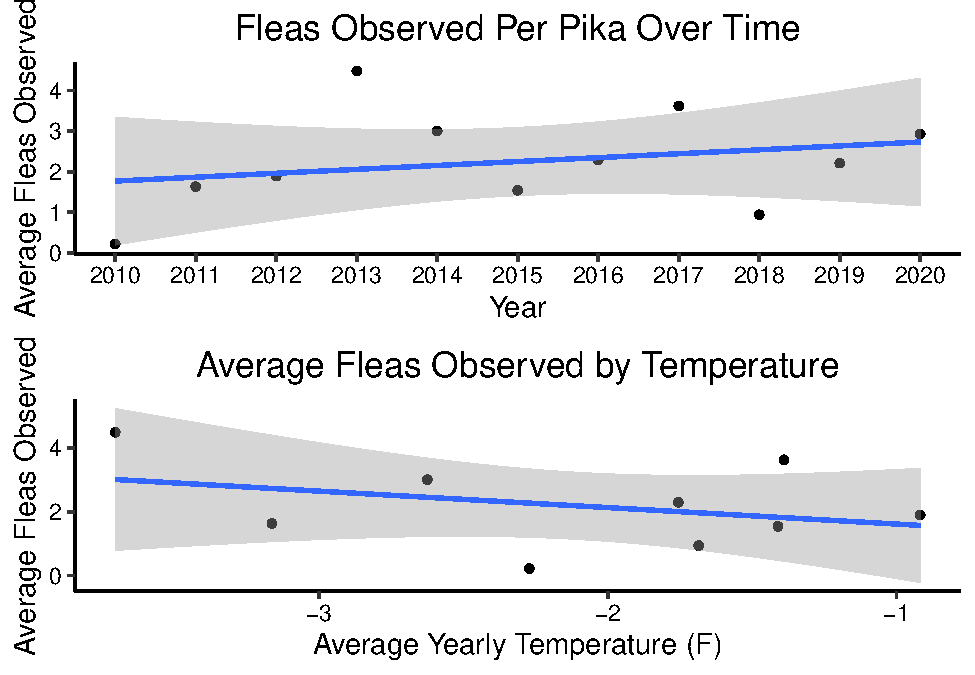
\includegraphics{FreedmanDye_ENV872_Project_files/figure-latex/unnamed-chunk-8-1.pdf}
\caption{Average number of fleas observed per year per pika over time
(top) and temperature (bottom).}
\end{figure}

Likewise, when regressions were run on the number of fleas sampled per
pika over time (linear model, F = 1.112, df = 10, Adjusted R-Square =
0.01005, p-value = 0.3165) and temperature (linear model, F = 0.3773, df
= 8, Adjusted R-Square = -0.07434, p-value = 0.5561), no significant
trends were found (Figure 10).

\begin{figure}
\centering
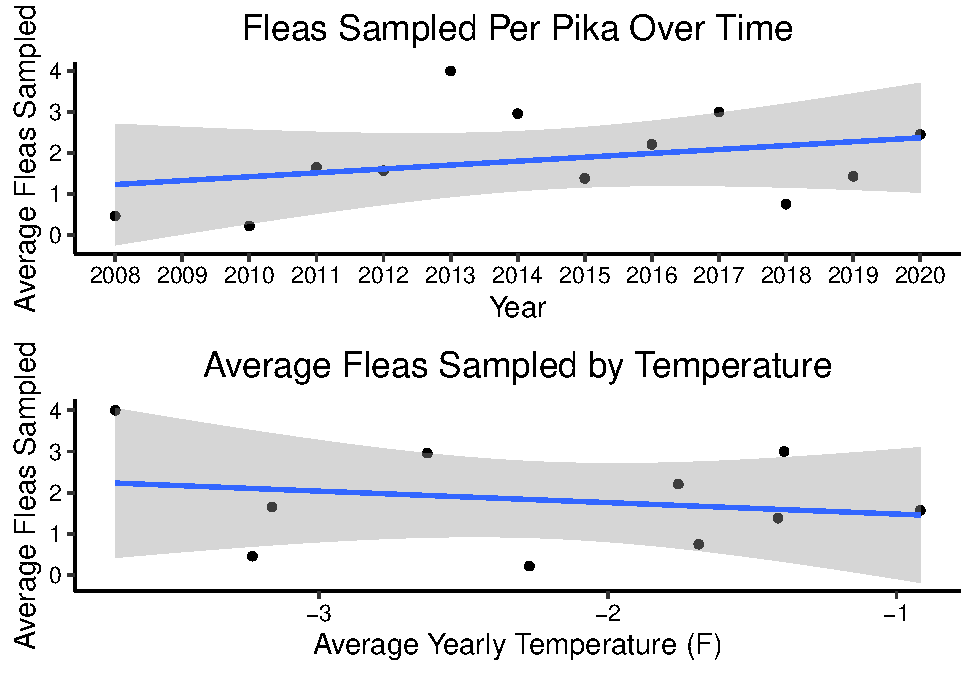
\includegraphics{FreedmanDye_ENV872_Project_files/figure-latex/unnamed-chunk-9-1.pdf}
\caption{Average number of fleas sampled per year per pika over time
(top) and temperature (bottom).}
\end{figure}

Finally, the proportion of captured pikas with ear mites present over
both time (linear model, F = 0.08857, df = 10, Adjusted R-Square =
-0.09034, p-value = 0.7721) and temperature (linear model, F = 0.1842,
df = 8, Adjusted R-Square = 0.08226, p-value = 0.2158) did not change
(Figure 11).

\begin{figure}
\centering
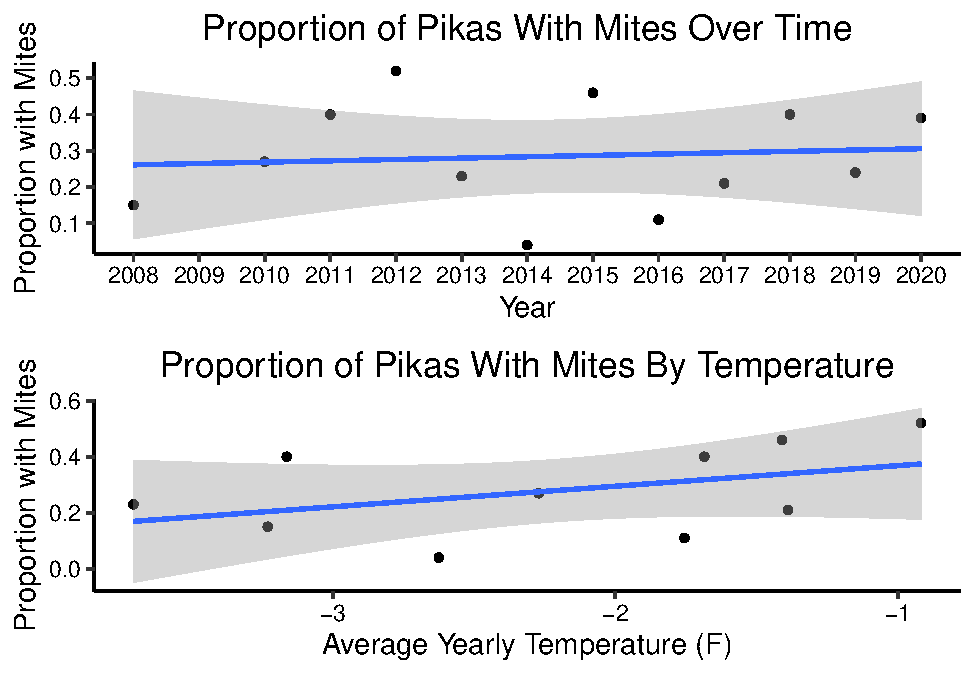
\includegraphics{FreedmanDye_ENV872_Project_files/figure-latex/unnamed-chunk-10-1.pdf}
\caption{Proportion of pikas with mites per year over time (top) and
temperature (bottom).}
\end{figure}

While no clear patterns were found for any of our tested variables, some
plots reveal the expected general trends. Fleas sampled, fleas observed,
and mites sampled visually increased over time (Figure 9,10,11).
However, when compared to temperature data, only the proportion of mites
present on captured pikas increased with increasing temperature. The
flea data trend lines decreased with increasing temperature. As shown in
figure 12, the ear mite observed categories had no perceivable pattern
that would indicate a correlation over time.

\begin{figure}
\centering
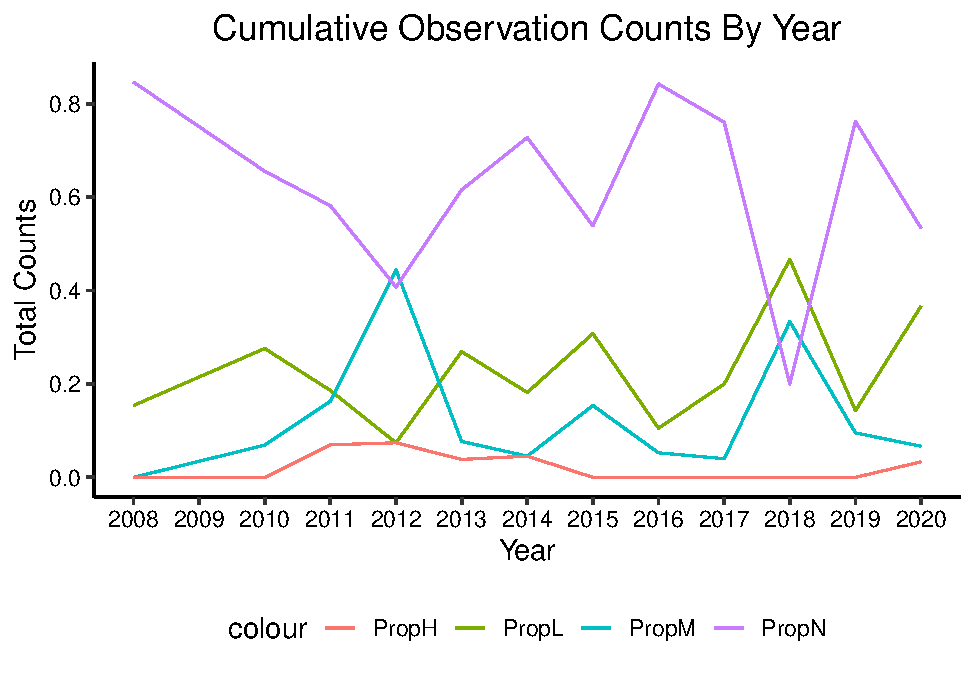
\includegraphics{FreedmanDye_ENV872_Project_files/figure-latex/unnamed-chunk-11-1.pdf}
\caption{Proportion of pikas with given mite density (PropN = None,
PropL = Low, PropM = Medium, PropH = High) over time.}
\end{figure}

\newpage

\hypertarget{summary-and-conclusions}{%
\section{Summary and Conclusions}\label{summary-and-conclusions}}

First and foremost, climate change is occurring at Niwot Ridge as
temperature has increased rapidly over the past 15 years. This was
expected not only because of climate change's impact on alpine regions,
but because the LTER climate dataset was very comprehensive. It was
valuable to have access to daily temperature values to run a time series
analysis that was built on thousands of data observations.

As detailed in our wrangling section, the Pika dataset was less complete
and contained far many fewer observations. It is possible that with more
observations and more complete tag information (many entries had to be
eliminated to avoid double-counting recaptures), a significant trend in
pika population over time would have been observed. It is understandable
that pika populations increased with temperature, but not time, as mean
annual temperature did not increase every year.

Further analysis is required to investigate the spatial changes in pika
distribution over time. Although sampling effort was roughly even
between years, it is likely that spatial patterns would be more clear if
a strict pika sampling protocol was followed. For example, greater
sampling effort at one location would skew the location of the mean
annual observation, and make patterns difficult to identify. Although it
was beyond the scope of this project, it would be valuable to analyze
population changes at each site, and determine if the highest altitude
site (West Knoll) provided better habitat for pikas than the other two
sites.

No parasitic data had a significant correlation when regressions were
run over time and temperature. This analysis indicates that, while it is
estimated that increased temperatures over time will lead to an increase
of parasites, this trend has not actualized over the last ten years
within the pika population sampled at NIWOT Ridge.

\newpage

\hypertarget{references}{%
\section{References}\label{references}}

American Pika. National Wildlife Federation. (n.d.). Retrieved December
8, 2022, from
\url{https://www.nwf.org/Educational-Resources/Wildlife-Guide/Mammals/American-Pika\#}:\textasciitilde:text=American\%20pikas\%20are\%20small\%2C\%20rodent,to\%20camouflage\%20them\%20among\%20rocks.

\end{document}
